\documentclass[english,report,10pt]{extarticle}
\usepackage[utf8]{inputenc}
\usepackage[fixed]{fontawesome5}
\usepackage{xcolor}
\usepackage{datetime}
\usepackage{tabularx}
\usepackage{ragged2e}

\definecolor{customred}{HTML}{ff0000}
\definecolor{customyellow}{HTML}{ffe33c}
\definecolor{custommagenta}{HTML}{ff28ff}
\definecolor{custompink}{HTML}{daa0db}
\definecolor{customgreen}{HTML}{a8dda8}
\definecolor{customblue}{HTML}{4c70f0}
\definecolor{highlight}{HTML}{768fcc}
\definecolor{linkcolour}{HTML}{866188}

\usepackage{pifont}
\newcommand{\dotred}{\textcolor{customred}{\ding{108}}\hspace{.5ex}}
\newcommand{\dotyellow}{\textcolor{customyellow}{\ding{108}}\hspace{.5ex}}
\newcommand{\dotpink}{\textcolor{custompink}{\ding{108}}\hspace{.5ex}}
\newcommand{\dotmagenta}{\textcolor{custommagenta}{\ding{108}}\hspace{.5ex}}
\newcommand{\dotgreen}{\textcolor{customgreen}{\ding{108}}\hspace{.5ex}}
\newcommand{\dotblue}{\textcolor{customblue}{\ding{108}}\hspace{.5ex}}

% for hyperlinks
\usepackage{hyperref}
\hypersetup{
    colorlinks=true,
    linkcolor=linkcolour,
    urlcolor=highlight
}

% set margin
\RequirePackage[margin=1.3in, top=.7in, bottom=1.0in]{geometry}


% for newline instead of \\ and \newline
\usepackage{parskip}

\usepackage{graphicx}
\graphicspath{ {./images/} }
\usepackage{subcaption}
\usepackage{wrapfig}
\usepackage{float}

% for generating toc with unnumbered sections
\newcommand*{\nsection}[1]{
    \section*{#1}
    \addcontentsline{toc}{section}{#1}
}
\newcommand*{\nsubsection}[1]{
    \vspace{3ex}
    \subsection*{#1}
    \addcontentsline{toc}{subsection}{#1}
}

\begin{document}

\title{Research Summary}
\author{Hieu Vu}
\maketitle

My interests lie in the broad topic of improving the modelling capability of Deep Learning models, which refers to anything related to: \textit{information and knowledge representation, novel architectures and modelling paradigms, learnable causality and reasoning, effective and efficient training methods, etc.} This includes but not limited to topics such as \textit{Multimodality, Modularity, Representation Learning, and Causal Deep Learning.} \\

However, working in the industry means that my research is heavily influenced by the requirements of my employer. Furthermore, my employer is not a research organization, thus guidance for research was limited which required me to develop my own methodology. The works presented here are my attempts to align my interests with my responsibility as an employee, along with my attempts to explore new areas to broaden my knowledge and refine my interests.\\

This document briefly describes some highlights of my research works. These came from my full-time job, my undergraduate thesis, and my personal projects. The works are categorized into two main sections: \textit{Information Extraction from business documents}, which is a focus of my full-time job and my undergraduate thesis, and \textit{Personal exploration}, which contains other topics that I dabbled in during my personal time.\\

A list of my arXiv and peer-reviewed publications can be found in my \href{https://scholar.google.com/citations?user=iRZlaI8AAAAJ}{Google Scholar profile}.

\vspace{15ex}
\tableofcontents

\newpage

\nsection{Information Extraction from business documents}

At work, my team and I helped clients extract key-value information from their business documents, thus, most of my research focused on this area.

\nsubsection{A Span Extraction Approach for Information Extraction on Visually-Rich Documents}
\textit{Accepted to DIL@ICDAR 2021 - Best Paper Award} \\
\textit{\url{https://arxiv.org/pdf/2106.00978.pdf}} \\

This work formulated the task of key-value information extraction from document images as a span extraction task and presented two following ideas:
\begin{itemize}
    \item A cross-lingual transfer learning method for adapting \href{https://arxiv.org/abs/1912.13318}{LayoutLM} to a low-resource language.

          \begin{itemize}
              \item LayoutLM (an extension of BERT for document images by taking into account visual and spatial information) was the new state-of-the-art method at the time, but it was pre-trained in English only.
              \item But our data is in Japanese, and we did not have the data nor the computation needed to pre-train the model from scratch.
              \item Thus, my idea was to swap the text embeddings of the English LayoutLM with those of a Japanese BERT (Fig. \ref{fig:cross-lingual-transfer}). Then continue to pretrain the model for a short amount of time on a much smaller dataset (17k compared with over 1M).
          \end{itemize}

          The hypothesis was that:
          \begin{itemize}
              \item Positional features are language-independent and can be shared across languages with alike reading order.
              \item Furthermore, the encoder layers are capable of capturing attention from both semantic and positional inputs.
          \end{itemize}

          \textit{This contribution was my original idea.}

          \begin{figure}[h!]
              \centering
              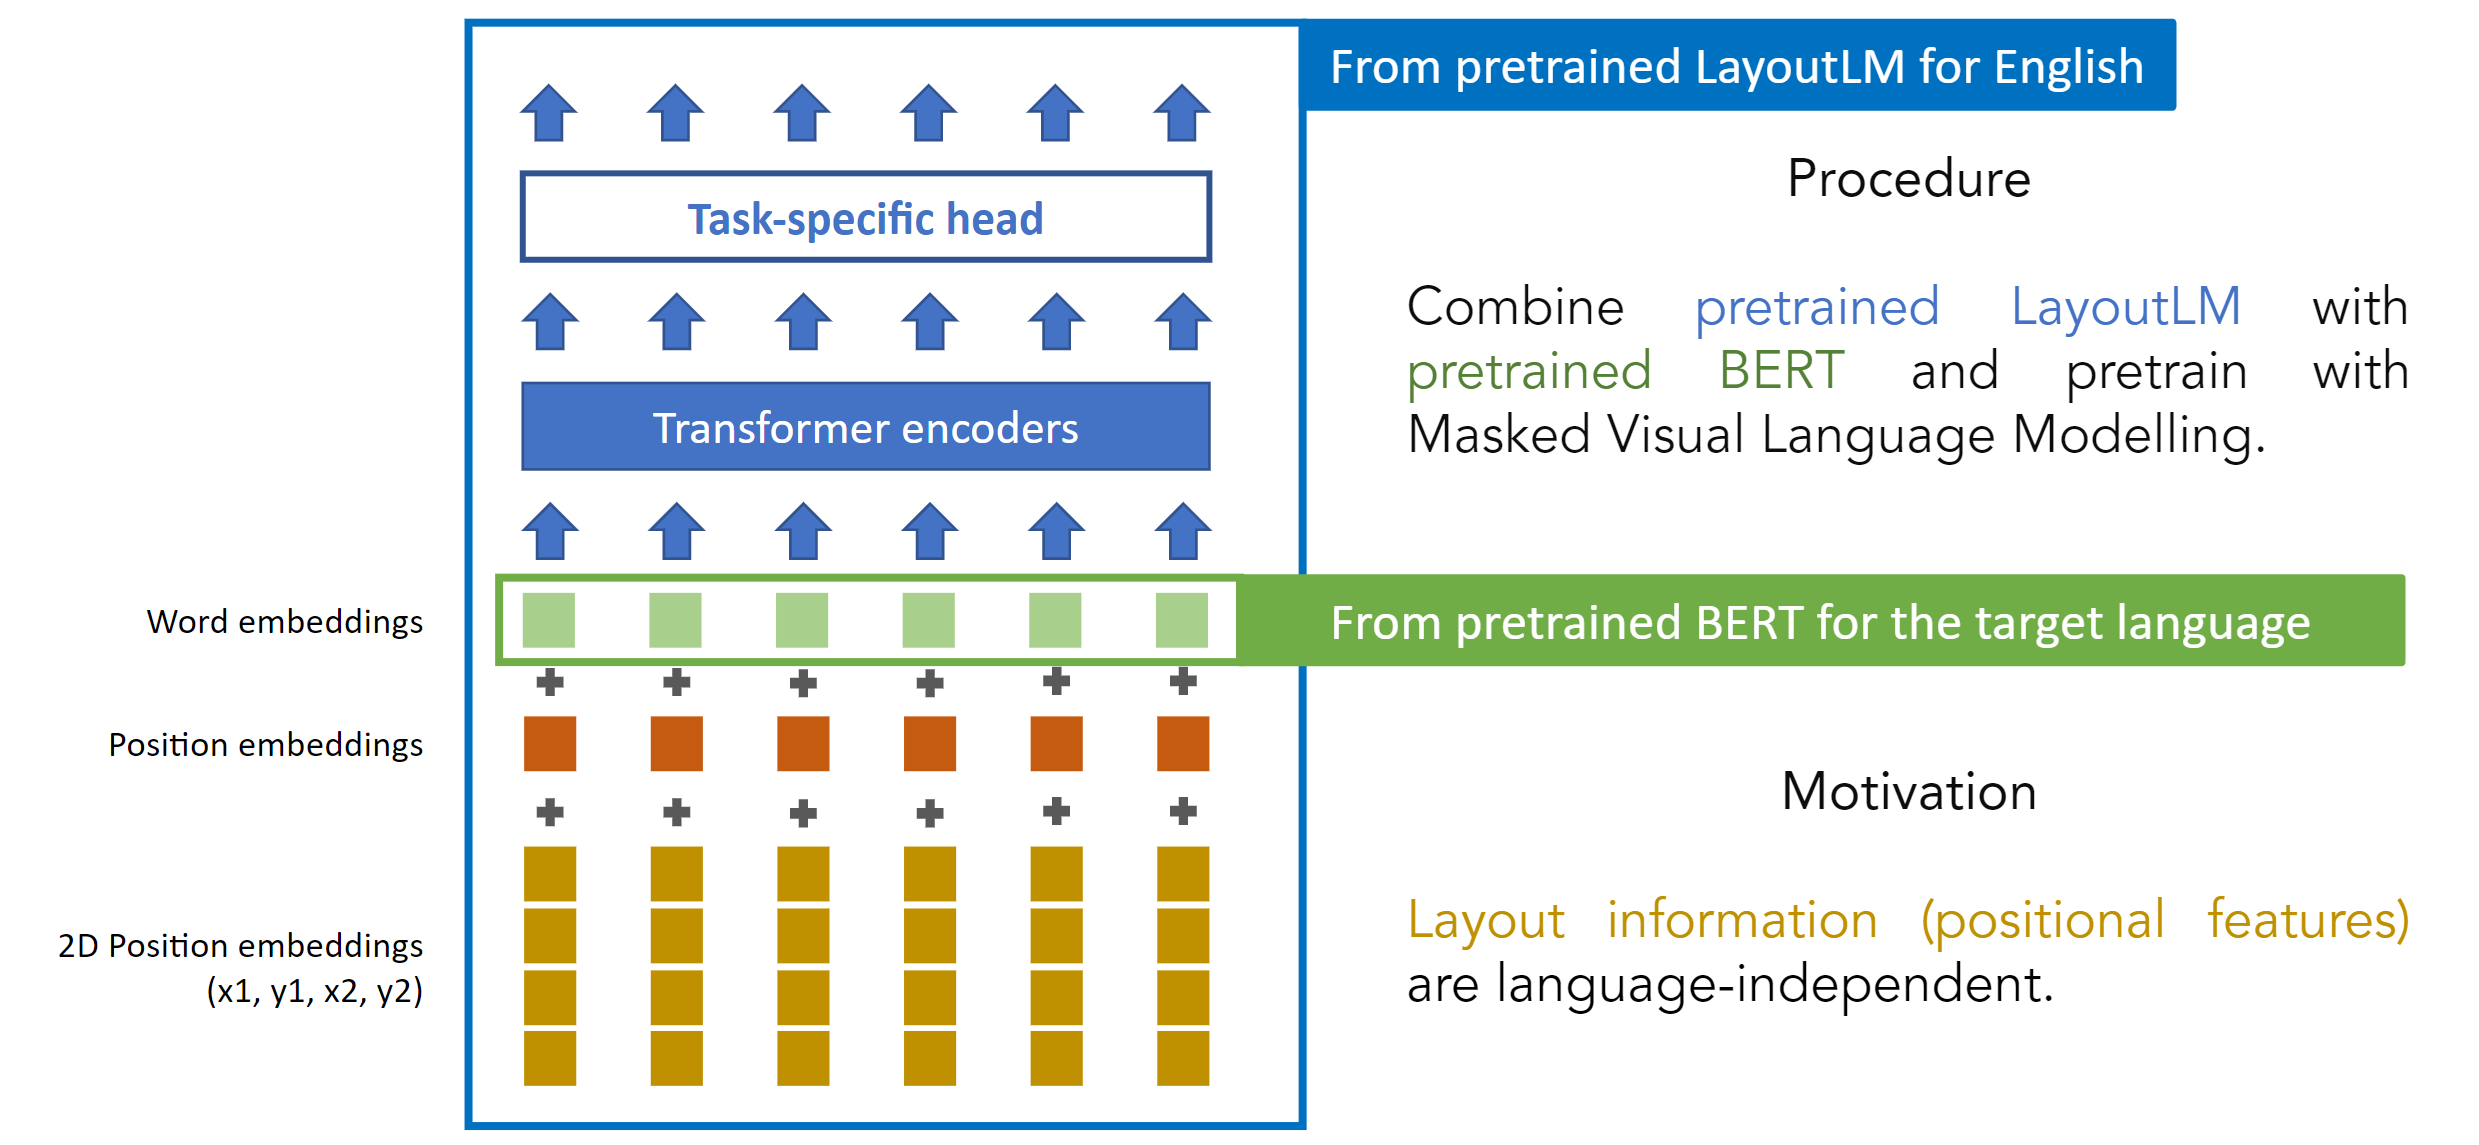
\includegraphics[width=14cm]{cross-lingual-transfer.png}
              \caption{Swapping LayoutLM's word embeddings with BERT's embeddings for cross-lingual transfer on a low-resource language.}
              \label{fig:cross-lingual-transfer}
          \end{figure}

    \item A recursive relation predicting scheme for multi-span extraction.

          One problem with span extraction is it only predicts a fixed number of spans for each query. However, in our case, there can be multiple different values for a single key information.

          This method addressed it by:
          \begin{itemize}
              \item Extracting the spans as a chain in a recursive manner.
              \item After the first span is extracted, the embeddings of its first token will be used as the query to extract the second span.
              \item The process continues until a stopping condition is reached (Fig. \ref{fig:recursive-span}).
          \end{itemize}

          This can be used both as a downstream task for multi-span extraction and also as a second-stage pretraining task.

          \begin{figure}[h!]
              \centering
              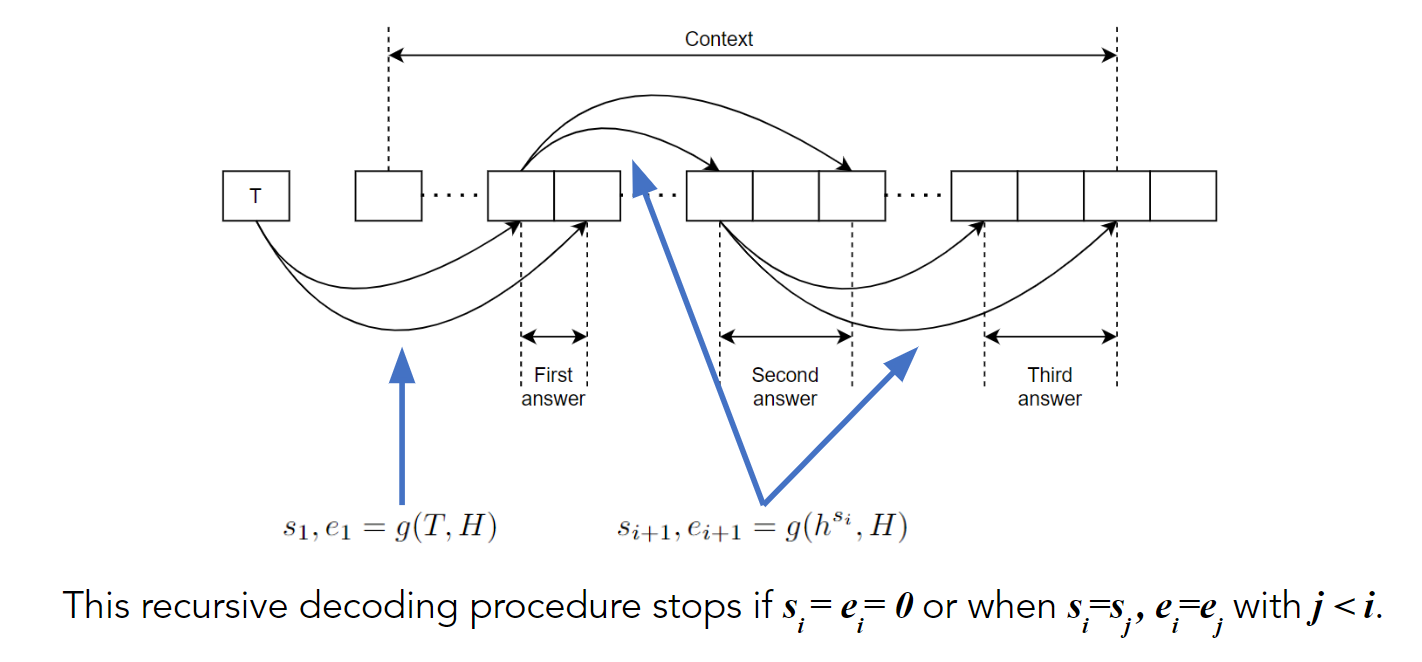
\includegraphics[width=14cm]{recursive-span.png}
              \caption{The recursive span extraction mechanism.}
              \label{fig:recursive-span}
          \end{figure}
\end{itemize}
\pagebreak


\nsubsection{Jointly Learning Span Extraction and Sequence Labeling for Information Extraction from Business Documents}
\textit{Accepted to IJCNN 2022 - Oral presentation} \\
\textit{\url{https://arxiv.org/pdf/2205.13434.pdf}} \\

This work aimed at the task of extracting multiple short-span key information from a long document. More specifically, it tried to address the following issues:

\begin{itemize}
    \item Due to the target information only making up a small portion of the document, a sequence labelling approach is affected by data imbalance.
    \item A span extraction approach is less affected by data imbalance, but it cannot extract multiple spans for a single key information. It also takes a long time to train and inference due to only being able to extract a single information at a time.
\end{itemize}

To this end, the paper proposed the following:

\begin{itemize}
    \item A query-based span extraction scheme that can process multiple queries at the same time.
          \begin{itemize}
              \item The queries refer to key information that needed to be extracted (e.g. \textit{contract date} or \textit{company name}).
              \item The queries are represented as learnt embeddings vectors.
              \item Then, attention scores are computed between the queries and the document.
              \item Finally, the attention scores are used to determine the start and end positions of the span.
          \end{itemize}

          This setup enables processing multiple queries at the same time, which reduces training and inference time significantly.

    \item Jointly learning span extraction and sequence labelling on two different branches, then combine the predictions.
          \begin{itemize}
              \item Since the above idea enables span extraction on multiple queries simultaneously just like sequence labelling, the model can perform sequence labelling on a parallel branch to get the best of both worlds.
              \item The sequence labelling branch allows the model to extract multiple values for each query.
              \item Furthermore, optimizing two downstream tasks simultaneously also improves the gradient, which contributes toward better performance and faster convergence.
          \end{itemize}

          \textit{This was my contribution to the methodology of this paper.}

\end{itemize}

\begin{figure}[h!]
    \centering
    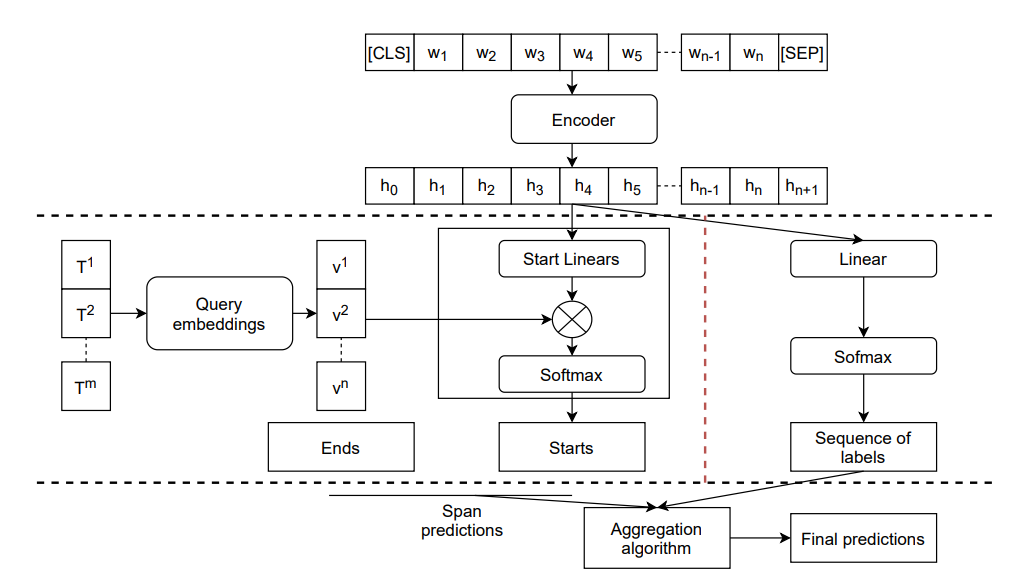
\includegraphics[width=10cm]{joint-span-seq.png}
    \caption{The proposed model, which jointly learns span extraction and sequence labelling.}
    \label{fig:joint-span-seq}
\end{figure}
\pagebreak


\nsubsection{A layout-aware key-value relation predicting model for document images}
\textit{Undergraduate thesis} \\
\textit{Advised by Dr. Diep Thi-Ngoc Nguyen} \\

My undergraduate thesis focused on detecting key and value regions in document images by formulating it as a segmentation problem. In which I presented the following:

\begin{itemize}
    \item A revised version of the \href{https://arxiv.org/abs/1905.13538}{FUNSD dataset}

          \begin{itemize}
              \item Upon inspecting the FUNSD dataset, I found it to be erroneous and have inconsistent labelling logic (An example is given in Fig. \ref{fig:funsd-vs-revised}).
              \item Thus I made the correction and published the revised version along with a report. The report is available at \url{https://arxiv.org/pdf/2010.05322.pdf}.
          \end{itemize}
          \begin{figure}[H]
              \centering
              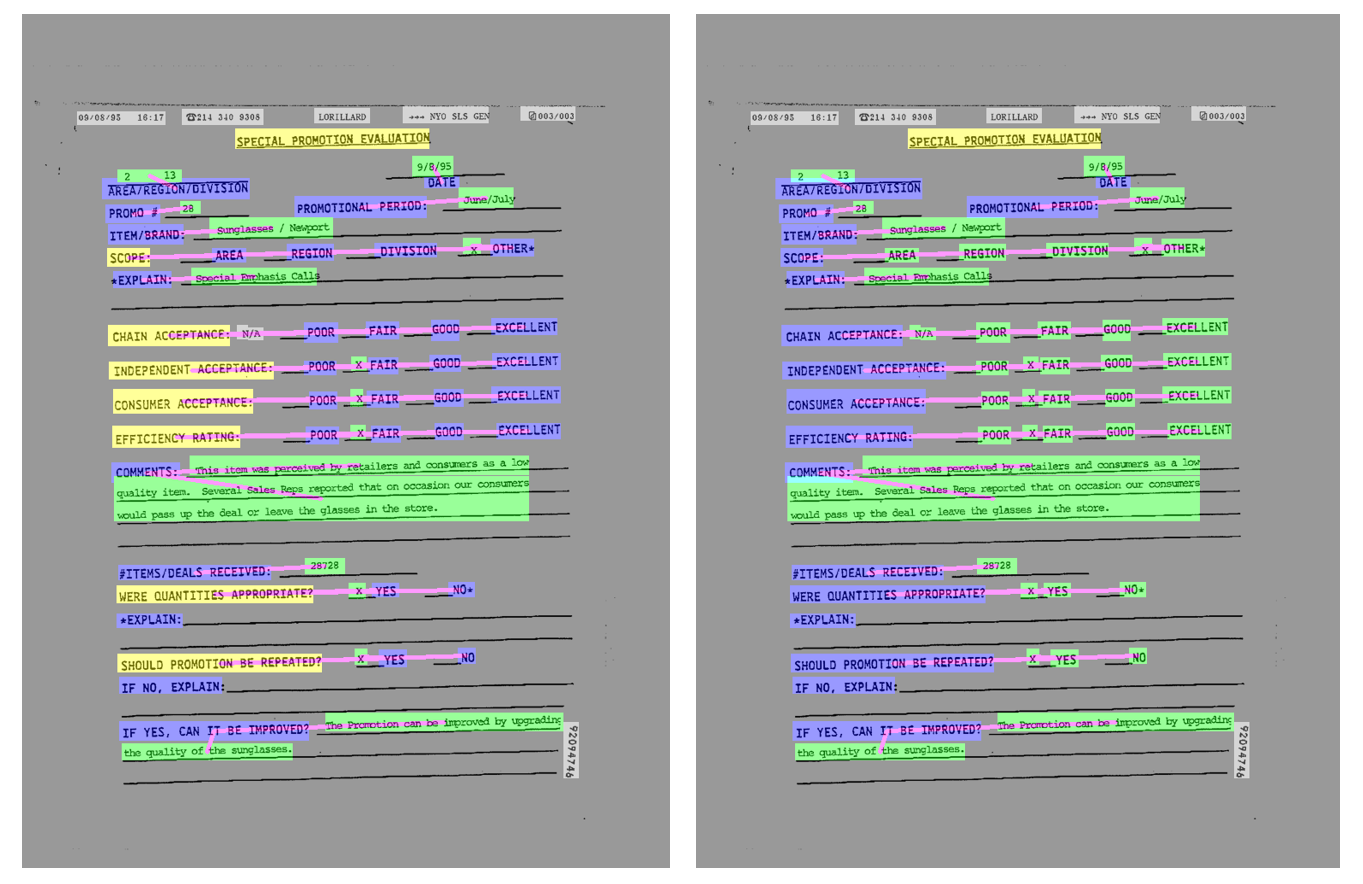
\includegraphics[width=0.7\textwidth]{funsd-vs-revised.png}
              \caption{A sample of from the FUNSD dataset (left) and its revised version. \dotyellow{} denotes \textit{headers}, \dotblue{} denotes \textit{questions}, \dotgreen{} denotes \textit{answers}, and \dotpink{} denotes the key-value relations.}
              \label{fig:funsd-vs-revised}
          \end{figure}

    \item A modified version (Fig. \ref{fig:ci-deform}) of \href{https://arxiv.org/abs/1703.06211}{Deformable Convolution} (Fig. \ref{fig:ori-deform}) where the convolution offsets stay the same for all channels.
          \begin{itemize}
              \item Learns only one set of offsets for all channels, keeping the channel-wise relation unchanged.
              \item Reduces the number of parameters significantly and improves processing time while still achieving comparable results.
          \end{itemize}

          \begin{figure}[h]
              \centering
              \begin{subfigure}{0.5\textwidth}
                  \centering
                  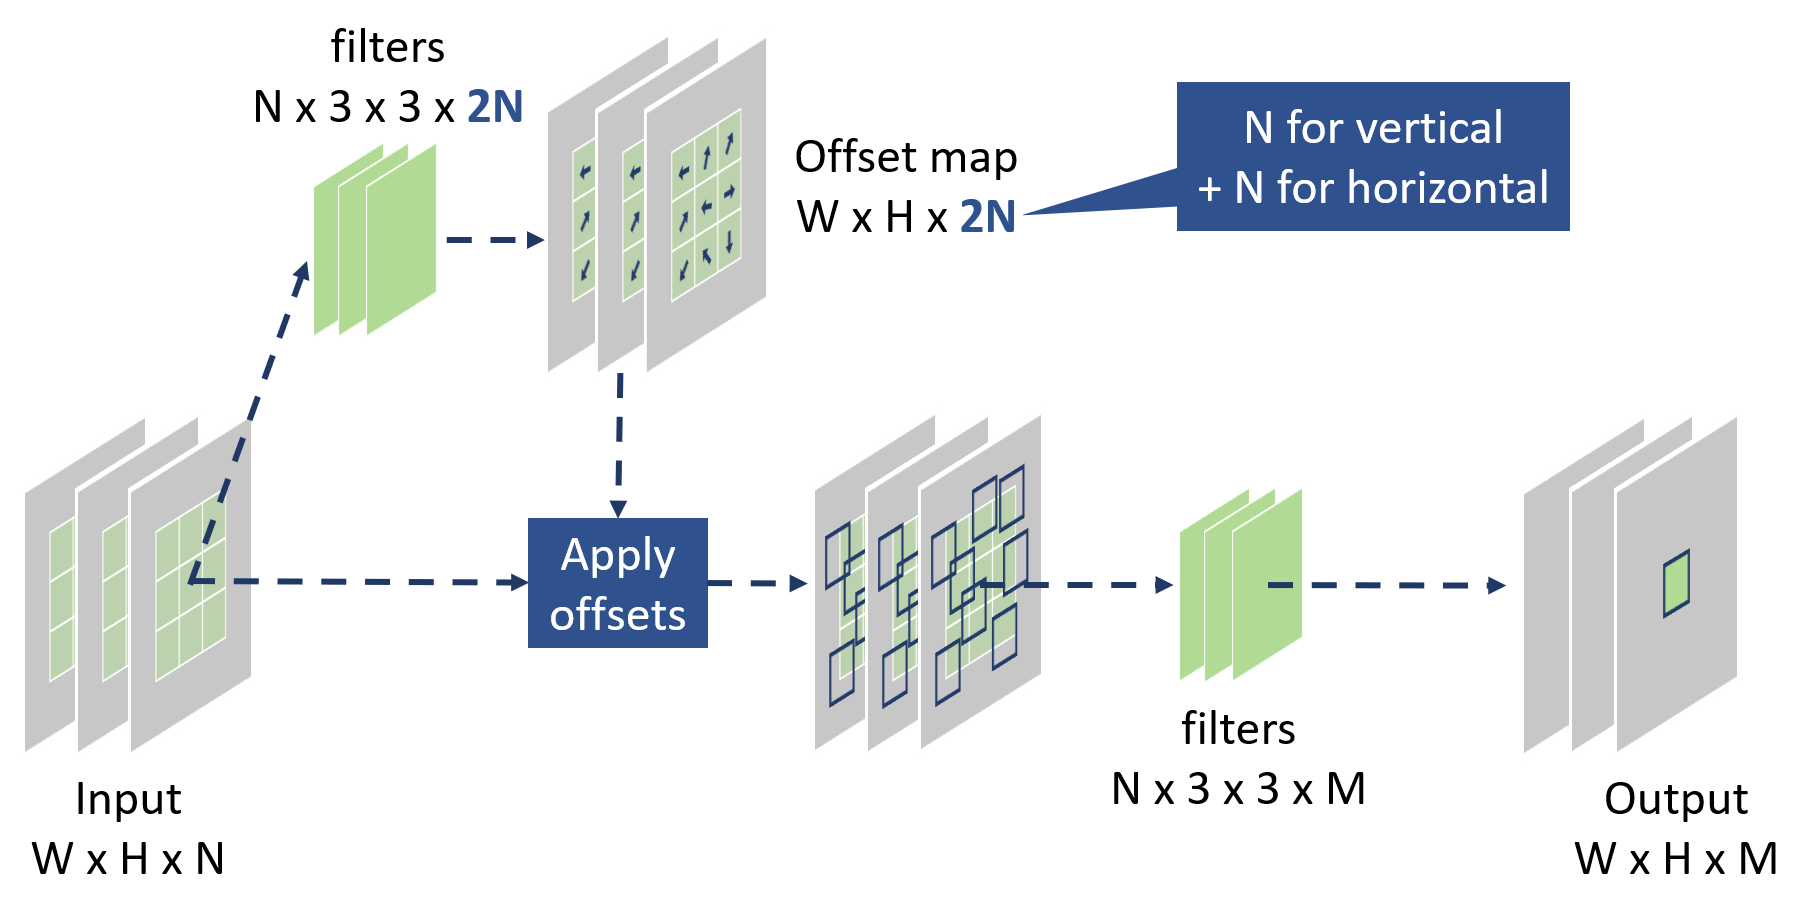
\includegraphics[width=0.9\linewidth]{deform-conv.png}
                  \caption{Deformable Convolution}\label{fig:ori-deform}
              \end{subfigure}%
              \begin{subfigure}{0.5\textwidth}
                  \centering
                  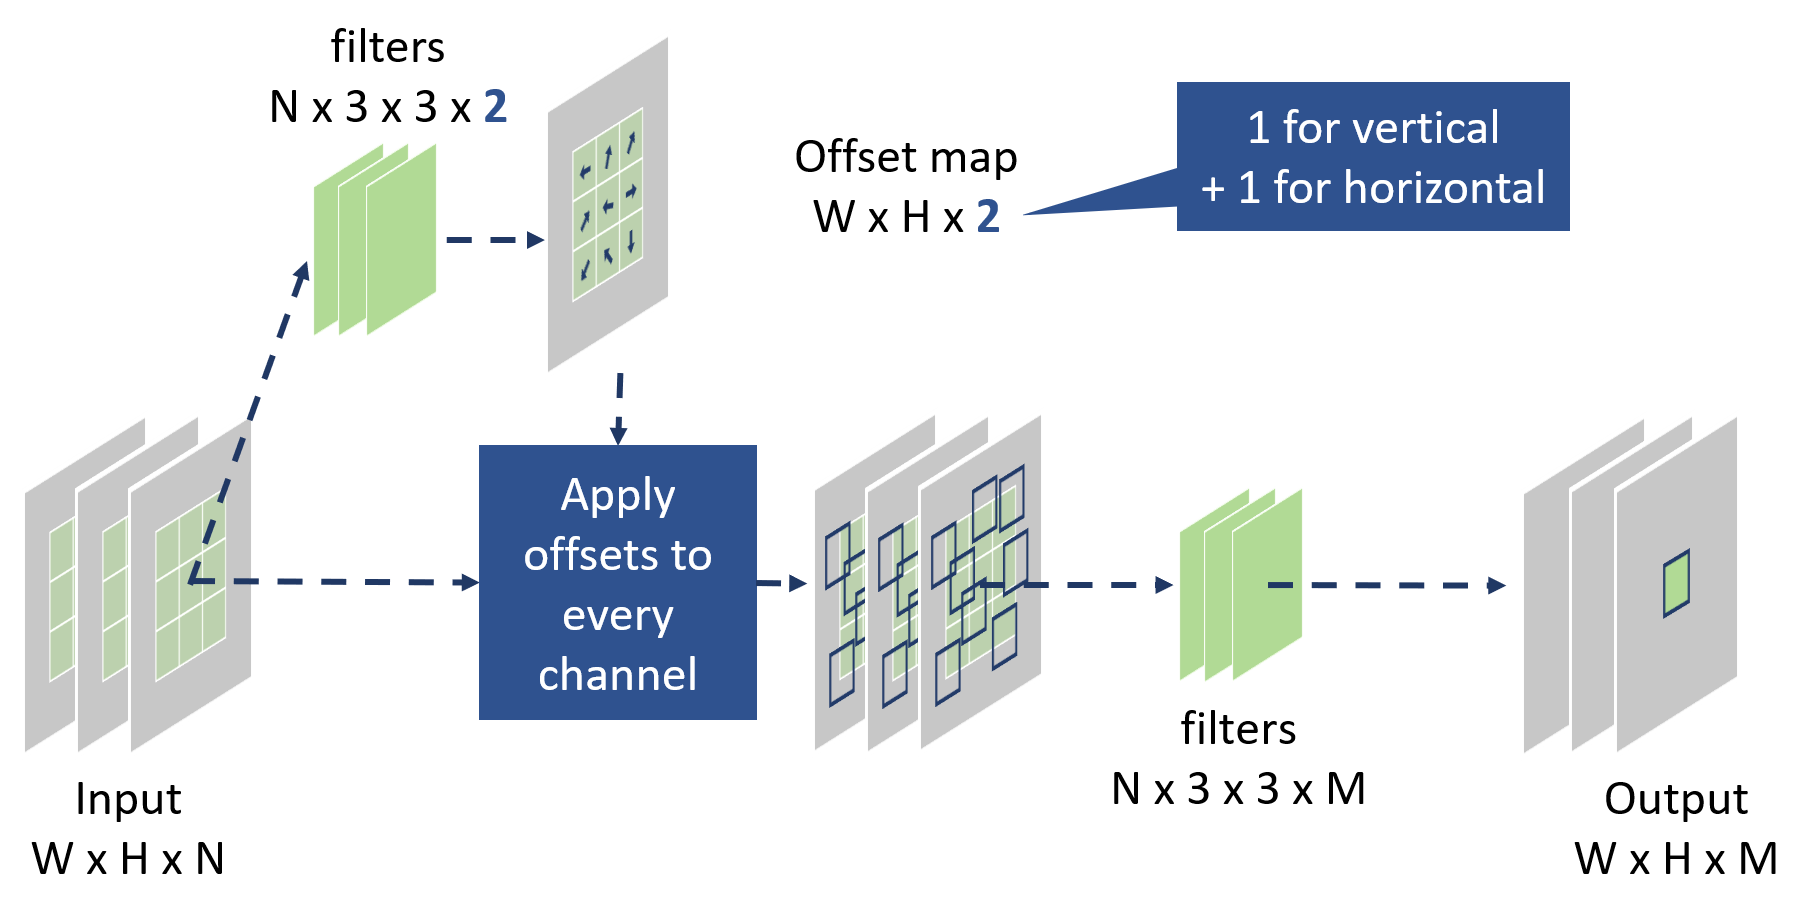
\includegraphics[width=0.9\linewidth]{ci-deform-conv.png}
                  \caption{Channel Invariant Deformable Convolution}\label{fig:ci-deform}
              \end{subfigure}
              \caption{Illustration of two $3x3$ Deformable Convolutions.}\label{fig:two-deform}
          \end{figure}

          \newpage
          The motivations were:
          \begin{itemize}
              \item Deformable Convolution is computationally expensive.
              \item Deformable Convolution learns the offset for each channel separately, thus the features in each channel will be sampled differently. This breaks the depth-wise invariant relation between channels but instead enhances the spatial relations within each channel.
              \item For classification tasks, this characteristic is preferable, as it enables each channel to embed entirely different information.
              \item But for segmentation tasks, it introduces unnecessary complexity.
          \end{itemize}
\end{itemize}
\pagebreak


\nsection{Personal exploration}

Apart from work-related topics, I tried to find opportunities to explore other areas for the purpose of learning new things and satisfying my curiosity. This also helps me expand my knowledge and be clearer about my interests.

\nsubsection{Learning Causal Inference and Improving DECAF}
\textit{\url{https://github.com/lone17/DECAF/blob/main/main.pdf}}\\

Causal Inference was a completely new topic that I discovered by chance. This field, along with Causal Discovery, gives me the thought that it could potentially help us build models with reasoning capability. I spent two weeks teaching myself the basics of Causal Inference and applied what I learnt to try to improve the paper \href{https://arxiv.org/abs/2110.12884}{DECAF: Generating Fair Synthetic Data Using Causally-Aware Generative Networks}.

DECAF is a method that aims to generate synthetic (and debiased) tabular data using a GAN-based model with an assumed causal DAG. The method consists of two stages:
\begin{itemize}
    \item First, given a DAG describing the underlying causal relation of the training data, a GAN-based model is trained to generate synthetic data by following the topology of the given DAG.
    \item During inference, a relaxed DAG is used to generate the data. The relaxed DAG is the original DAG  with some edges removed to eliminate the causal relation between the protected attributes and the target attributes, which increases fairness.
\end{itemize}

Another aspect that DECAF is concerned with is data utility, which is the measure of how similar the synthetic data is to the original (biased) data. Naturally, there is a trade-off between data utility and fairness. My work attempted to improve the data utility of DECAF while still achieving a similar level of fairness. More specifically, it proposed:
\begin{itemize}
    \item A a new relaxed DAG (with different relaxation logics) to generate the target attribute (An example for the \textit{income} attribute of the \href{https://archive.ics.uci.edu/dataset/2/adult}{Adult dataset} is given in Fig. \ref{fig:edge-removal-target}).
    \item Alternating between the DECAF's relaxed DAG and the new relaxed DAG to maximize the information flow to the target attribute while not violating any d-separation constraints.
    \item Some metrics to measure the trade-off between data utility and fairness.
\end{itemize}

\begin{figure}[!h]
    \centering
    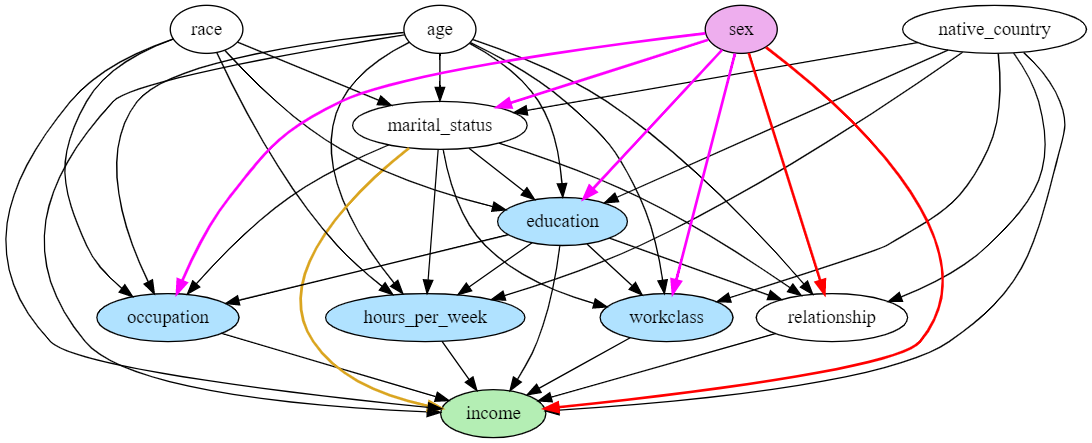
\includegraphics[width=0.9\linewidth]{edge-removal-target.png}
    \caption{(The same example in Figure 6 of the DECAF paper) DAG for generating \textit{income} in the Adult dataset. The target variable is in \textcolor{customgreen}{green}, the protected attribute in \textcolor{custompink}{pink}, and the allowed Conditional Fairness variables in \textcolor{customblue}{blue}. \textit{Demographic Parity} is achieved by removing: \dotred\dotyellow\dotmagenta; \textit{Conditional Fairness} is achieved by removing: \dotred\dotyellow.}
    \label{fig:edge-removal-target}
\end{figure}
\pagebreak


\nsubsection{Inferring Properties of Graph Neural Network and Defending Against Backdoor Attacks}
\textit{A work of a friend that I contributed to.}\\
\textit{\url{https://arxiv.org/abs/2401.03790}}\\

My friend, who is a PhD Candidate at The University of Melbourne, needed a hand with his research, so I joined to help him and also to have a chance to gain knowledge on GNNs and backdoor attacks.

\begin{figure}[h!]
    \centering
    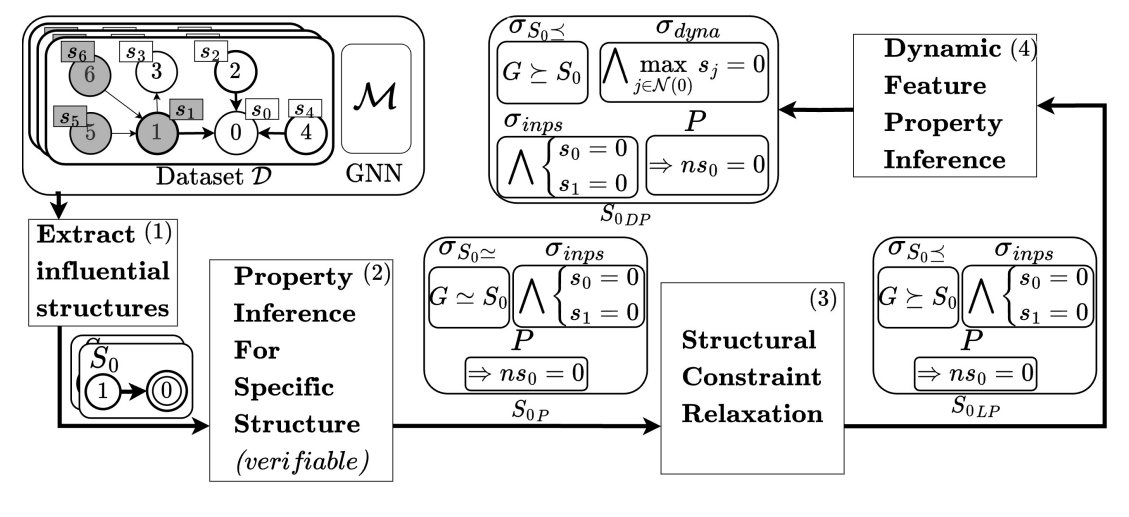
\includegraphics[width=14cm]{gnn-infer.png}
    \caption{GNN-Infer overview.}
    \label{fig:gnn-infer}
\end{figure}

The work proposed \textit{GNN-Infer}, a new method for automatic property inference technique of GNNs, and applied it to detecting and defending against backdoor attacks. The method comprises 4 stages (as illustrated in Fig. \ref{fig:gnn-infer}):
\begin{itemize}
    \item \textit{Extract influential structures}
          \begin{itemize}
              \item Analyzes the trained GNN and the training data and outputs influential structures.
              \item Influential structures are subgraphs that frequently appear in the dataset and significantly impact GNN predictions.
          \end{itemize}
    \item \textit{Property inference for each specific structure}
          \begin{itemize}
              \item For each influential structure, turn it into the equivalent feed-forward network (FNN). This was done because there is no known property inference method for GNNs due to its dynamic nature.
              \item Infers the properties of the FNN using existing techniques.
              \item The properties are rules that describe the future state of the target node based on the current state of connected nodes.
          \end{itemize}
    \item \textit{Structure constraints relaxation}
          \begin{itemize}
              \item Generalizes each structure-specific property to a \textit{subgraph isomorphic} (i.e. graphs that contain the same subgraph) property, covering a broader set of input graphs.
              \item These properties are more general and useful, but they are just \textit{likely properties} as they cover dynamic structures.
          \end{itemize}
    \item \textit{Dynamic Property Inference}.
          \begin{itemize}
              \item Augments the \textit{likely properties} with dynamic feature properties.
              \item Those are properties that consider the aggregated states of nodes in the full graph that are connected to the target node (as opposed to only considering connected nodes in the subgraph).
          \end{itemize}
\end{itemize}

For defending against backdoor attacks, the method is applied as follows:
\begin{itemize}
    \item Given a (poisoned) GNN and its training data, it infers the properties.
    \item Decides which properties are likely to be triggers based on their noticeability, stealthiness and effectiveness.
    \item Then prunes those properties from the GNN.
    \item The defence mechanism is effective if it reduces the Attack Success Rate of the attack while maintaining the Accuracy on the clean test set.
\end{itemize}

\textit{I contributed to the design and engineering of experiments for backdoor defence.}

\end{document}
